% concatenated from Geher_Pach_Swanepoel_Toth_On_the_number_of_edges_of_restricted_matchstick_graphs.tex
\documentclass[12pt]{article}

\usepackage{amssymb, amsmath, amsthm, graphicx}
\usepackage[left=1in,top=1in,right=1in]{geometry}
\usepackage[color=Orange!50!white, textwidth=22mm]{todonotes}

\usepackage{pgfplots}
\pgfplotsset{compat=1.15}
\usepackage{mathrsfs}
\usetikzlibrary{arrows}


\date{}
\setlength {\marginparwidth }{2cm} 
\theoremstyle{plain}
      \newtheorem{theorem}{Theorem}
      \newtheorem{lemma}[theorem]{Lemma}
      \newtheorem{claim}[theorem]{Claim}
      \newtheorem{problem}{Problem}
      \newtheorem{observation}[theorem]{Observation}
      \newtheorem{corollary}[theorem]{Corollary}
      \newtheorem{proposition}[theorem]{Proposition}
      \newtheorem{conjecture}[theorem]{Conjecture}
\theoremstyle{definition}
      \newtheorem{definition}{Definition}

\theoremstyle{remark}
      \newtheorem{remark}[theorem]{Remark}

\def\marrow{{\boldmath {\marginpar[\hfill$\rightarrow \rightarrow$]{$\leftarrow \leftarrow$}}}}



\title{On the number of edges of restricted matchstick graphs }
\author{Panna Geh\'er\thanks{E\"otv\"os University, Budapest, Hungary and Alfr\'ed R\'enyi Institute of Mathematics, Budapest, Hungary. Email: \texttt{geher.panna@ttk.elte.hu}.}
\and J\'anos Pach\thanks{Alfr\'ed R\'enyi Institute of Mathematics, Budapest, Hungary. Email: \texttt{pach@renyi.hu}.}
\and Konrad Swanepoel \thanks{Department of Mathematics, London School of Economics and Political Science. \newline Email: \texttt{k.swanepoel@lse.ac.uk}.}
\and G\'eza T\'oth\thanks{Alfr\'ed R\'enyi Institute of Mathematics, Budapest, Hungary. Email: \texttt{geza@renyi.hu}.}}

\begin{document}


\maketitle


\begin{abstract}

A graph whose vertices are points in the plane and whose edges are noncrossing straight-line segments of unit length is called a \emph{matchstick graph}. We prove two somewhat counterintuitive results concerning the maximum number of edges of such graphs in two different scenarios.

First, we show that there is a constant $c>0$ such that every triangle-free matchstick graph on $n$ vertices has at most $2n-c\sqrt{n}$ edges. This statement is not true for any $c>\sqrt2.$

We also prove that for every $r>0$, there is a constant $\varepsilon(r)>0$ with the property that every matchstick graph on $n$ vertices contained in a disk of radius $r$ has at most $(2-\varepsilon(r))n$ edges.
 

\end{abstract}

\section{Introduction}

Planar graphs have several interesting characterizations. One of them is given by the \mbox{so-called} circle packing theorem, also known as the Koebe--Andreev--Thurston theorem. It states that any planar graph can be realized by a set of circular disks in the following way: each disk represents a vertex, and two disks touch each other if and only if there is an edge connecting the two corresponding vertices of the graph. The number of edges that a planar graph on $n \geq 3$ vertices can have is at most $3n- 6$. This bound is tight with the extremal graphs being triangulations (planar graphs in which every face is bounded by a cycle of length $3$). However, the set of disks realizing a triangulation (with $n > 3$ vertices) necessarily contains disks of different radii. This motivates the following definition. A graph is called a \emph{penny graph} if it can be realized by a set of unit disks. Equivalently, a penny graph is a graph that can be drawn in the plane such that all edges are drawn as unit segments and the unit distance is the smallest distance among the vertices.

How can one determine the maximum number of edges of a penny graph on $n$ vertices? It is easy to see that every vertex has degree at most six, and also that not all vertices can be of degree six. If we call the vertices of degree smaller than six \emph{boundary points}, then it is not hard to argue, using the isoperimetric inequality, that there are at least $c\sqrt n$ boundary points, for some constant $c>0$ \cite{E46}.
Harborth \cite{Harborth74} proved that a penny graph on $n$ vertices can have at most $\lfloor 3n - \sqrt{12n - 3}\rfloor$ edges. His result is tight, as is demonstrated by a hexagonal piece of the regular triangular lattice.

Harborth later conjectured \cite{Harborth2} that his result holds for the larger graph class of so-called matchstick graphs (introduced by him in 1981 \cite{Harborth1}). \emph{Matchstick graphs} are plane unit-distance graphs; in other words, they can be drawn such that the vertices are represented by points in the plane, and the edges are non-crossing straight-line segments of unit length.
These graphs are much harder to handle than penny graphs.
For instance, unlike penny graphs, there is no upper bound for the maximum degree of the vertices of a matchstick graph, which made it much more difficult to prove Harborth's conjecture. After almost 40 years, the problem was recently settled by Lavoll\'ee and Swanepoel \cite{LS22}. The main idea of their proof is the following. If a matchstick graph has more than $3n-\sqrt{12n-3}$ edges, then almost all of its vertices must have degree $6$ and almost all faces must be triangular. Since all triangular faces are necessarily equilateral triangles, the area of the union of the bounded faces is bounded from below by $\Omega(n)$. By the isoperimetric inequality, the union of the unbounded faces has perimeter at least $\Omega(\sqrt{n})$, which means that there must be $\Theta(\sqrt{n})$ boundary points. Then it is shown that in an optimal configuration, a large part of the vertex set must lie on a triangular lattice. Then a modified isoperimetric inequality (a form of Lhuilier's inequality) is applied to show that the whole graph must lie on a triangular lattice. 

In this paper we consider two further problems about matchstick graphs that turn out to be much harder than they appear, and the solutions are somewhat counterintuitive.

Penny graphs and matchstick graphs with a maximum number of edges contain many triangles. It is an intriguing problem to determine the maximum number of edges that \emph{triangle-free} penny graphs and matchstick graphs with $n$ vertices can have. For the case of penny graphs, this question was first considered by Swanepoel \cite{S09}. He conjectured that the maximal number of edges of a triangle-free penny graph on $n$ vertices is $2n - 2 \sqrt n$. Apart from finding a non-trivial constant factor on the square-root term in \cite{E17}, this conjecture is still open.
The analogous question for matchstick graphs is also open, but has a different nature.

\begin{problem} \label{problem_trianglefree}
Determine or estimate the maximum number of edges $e(n)$ that a triangle-free matchstick graph on $n$ vertices can have.
\end{problem}

Again, using Euler's formula, we obtain that $e(n) \leq 2n-4$, and this bound is tight for triangle-free planar graphs. For matchstick graphs, we expect to obtain a better bound. In the absence of triangles, every face of a matchstick graph has at least four sides. Since there is no positive lower bound for the area of such faces, one cannot directly use  isoperimetric inequalities.
We might conjecture, as in the case of triangle-free penny graphs \cite{S09}, that, if $n$ is a perfect square, then the maximum number of edges is attained  by a $\sqrt n \times \sqrt n$ piece of the integer lattice (see Figure \ref{fig_grid}), in which case the maximum would be $2n-2\sqrt{n}-O(1)$. Our first theorem shows that this is not the case. In particular, there is a better lower bound than the square grid.

\begin{figure}[h!]
\centering

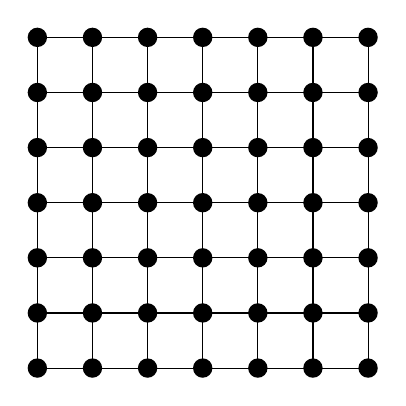
\begin{tikzpicture}[scale=0.7]
\foreach \x in {1,...,7} {
    \foreach \y in {1,...,7} {
        \fill (\x,\y) circle (5pt);
    }
}

\foreach \x in {1,...,7} {
\draw (\x, 1) --  (\x, 7); 
\draw (1, \x) --  (7, \x); 
}


\end{tikzpicture}

\caption{The $\sqrt n \times \sqrt n$ piece of the integer lattice defines a triangle-free matchstick graph with $n$ vertices and $2n-2\sqrt{n}-O(1)$ edges.}
\label{fig_grid}
\end{figure}


\begin{theorem}\label{thm1}
The maximum number of edges $e(n)$ in a triangle-free matchstick graph on $n$ vertices satisfies
\[ 2n-\sqrt{2}\sqrt{n}-O(1) \leq e(n)\leq 2n-\frac{\sqrt{2}}{5}\sqrt{n}.    \]
\end{theorem}


A different constraint that we can put on a matchstick graph is that it must be contained in some fixed bounded region, such as a disk of radius $r$. Note that the diameter of the best known constructions for Problem \ref{problem_trianglefree} tends to infinity, as $n$ tends to infinity. However, for every $n$, it is easy to construct triangle-free unit distance graphs with $n$ vertices and $(1+c)n$ edges in a disk of fixed radius $r$, where $c=c(r) > 0$ (see Proposition~\ref{lower_bound}). The following question arises.

\begin{problem} \label{problem_boundedmatchstick}
For any fixed $r>0$, let $e_{r}(n)$ be the maximum number of edges of a matchstick graph on $n$ vertices contained in a
disk of radius $r$. 

For a given $r>0$, determine $e_{r}(n)$ or at least its asymptotic behaviour, as $n\rightarrow\infty.$ 
\end{problem}


Since the number of triangles has to be bounded by a constant depending on $r$, Euler's formula implies an upper bound of $2n+O_r(1)$ for the number of edges. Our second theorem shows that, again surprisingly, the answer is substantially
smaller than $(2-o(1))n$.

\begin{theorem}\label{boundedmatchstick}
For any $r>0$, there are $c_1(r), \, c_2(r)>0$ such that for any $n>0$, we have
\[\left(2-c_1(r)\right)n\le e_r(n)\le \left(2-c_2(r)\right)n.\]

In particular, the statement holds with 
$c_1(r)=5/r+o(1)$ and $c_2(r)=20/3^{16r^2}$.
\end{theorem} 

The dependency of $c$ on $r$ in the upper bound is probably far from the truth, while the lower bound is probably close to the optimal value.


\section{Triangle-free matchstick graphs}
In this section, we prove Theorem~\ref{thm1}.
We first consider the lower bound.


\begin{proposition}\label{prop:triangle-free-lower-bound}
For each $n$ there exists a triangle-free matchstick graph on $n$ vertices with $\left\lfloor 2n-\sqrt{2n-\frac{7}{4}}-\frac{3}{2}\right\rfloor$ edges.
\end{proposition}

\begin{proof}[Proof sketch.]
A regular $2k$-gon (or more generally, a convex centrally symmetric $2k$-gon) with unit side lengths can be tiled by $\binom{k}{2}$ rhombi to create a matchstick graph with $n=\binom{k+1}{2}+1$ vertices and $e=k^2$ edges.
(See Figure~\ref{fig:tiling} for the case $k=4$.)
For these values of $n$ and $e$ we have $e= 2n-\sqrt{2n-\frac{7}{4}}-\frac{3}{2}$.
For values of $n$ between $\binom{k+1}{2}+1$ and $\binom{k+2}{2}+1$ we can build around the boundary to attain $\left\lfloor 2n-\sqrt{2n-\frac{7}{4}}-\frac{3}{2}\right\rfloor$ edges, as in Figure~\ref{fig:tiling}.
\begin{figure}[h]
\begin{center}
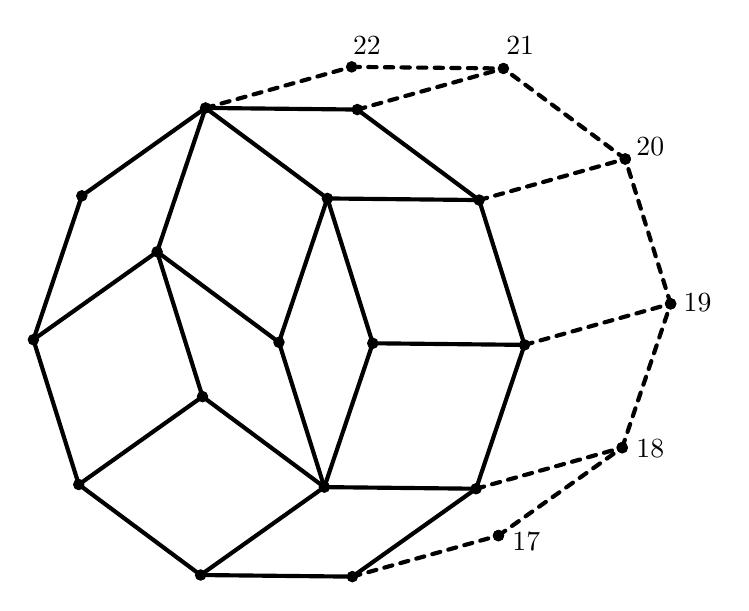
\begin{tikzpicture}[line cap=round,line join=round,>=triangle 45,scale=0.75]
\draw [line width=1.5pt] (-6.645005805614367,5.3115128748036335)-- (-4.55,6.8);
\draw [line width=1.5pt] (-4.55,6.8)-- (-3.730015480361444,9.235624896199406);
\draw [line width=1.5pt] (-3.730015480361444,9.235624896199406)-- (-4.4982584629518705,11.688061636899114);
\draw [line width=1.5pt] (-4.4982584629518705,11.688061636899114)-- (-6.56128624004033,13.220562742410849);
\draw [line width=1.5pt] (-6.56128624004033,13.220562742410849)-- (-9.131092320514174,13.247764878225915);
\draw [line width=1.5pt] (-9.131092320514174,13.247764878225915)-- (-11.22609812612854,11.759277753029549);
\draw [line width=1.5pt] (-11.22609812612854,11.759277753029549)-- (-12.046082645767097,9.323652856830144);
\draw [line width=1.5pt] (-12.046082645767097,9.323652856830144)-- (-11.277839663176671,6.8712161161304355);
\draw [line width=1.5pt] (-11.277839663176671,6.8712161161304355)-- (-9.214811886088212,5.3387150106187);
\draw [line width=1.5pt] (-9.214811886088212,5.3387150106187)-- (-6.645005805614367,5.3115128748036335);
\draw [line width=1.5pt] (-12.046082645767097,9.323652856830144)-- (-9.95107684015273,10.81213998202651);
\draw [line width=1.5pt] (-9.95107684015273,10.81213998202651)-- (-9.131092320514174,13.247764878225915);
\draw [line width=1.5pt] (-9.95107684015273,10.81213998202651)-- (-7.888049063064271,9.279638876514776);
\draw [line width=1.5pt] (-7.888049063064271,9.279638876514776)-- (-7.068064543425715,11.71526377271418);
\draw [line width=1.5pt] (-7.068064543425715,11.71526377271418)-- (-9.131092320514174,13.247764878225915);
\draw [line width=1.5pt] (-7.068064543425715,11.71526377271418)-- (-4.4982584629518705,11.688061636899114);
\draw [line width=1.5pt] (-7.068064543425715,11.71526377271418)-- (-6.299821560835288,9.262827032014473);
\draw [line width=1.5pt] (-6.299821560835288,9.262827032014473)-- (-3.730015480361444,9.235624896199406);
\draw [line width=1.5pt] (-6.299821560835288,9.262827032014473)-- (-7.119806080473845,6.8272021358150665);
\draw [line width=1.5pt] (-7.119806080473845,6.8272021358150665)-- (-7.888049063064271,9.279638876514776);
\draw [line width=1.5pt] (-9.95107684015273,10.81213998202651)-- (-9.182833857562304,8.359703241326802);
\draw [line width=1.5pt] (-9.182833857562304,8.359703241326802)-- (-7.119806080473845,6.8272021358150665);
\draw [line width=1.5pt] (-9.182833857562304,8.359703241326802)-- (-11.277839663176671,6.8712161161304355);
\draw [line width=1.5pt] (-9.214811886088212,5.3387150106187)-- (-7.119806080473845,6.8272021358150665);
\draw [line width=1.5pt] (-7.119806080473845,6.8272021358150665)-- (-4.55,6.8);
\draw [line width=1.5pt,dashed] (-6.645005805614367,5.3115128748036335)-- (-4.170932083018117,6.006928191425282);
\draw [line width=1.5pt,dashed] (-2.0759262774037506,7.495415316621648)-- (-1.2559417577651946,9.931040212821054);
\draw [line width=1.5pt,dashed] (-4.170932083018117,6.006928191425282)-- (-2.0759262774037506,7.495415316621648);
\draw [line width=1.5pt,dashed] (-1.2559417577651946,9.931040212821054)-- (-2.0241847403556212,12.383476953520763);
\draw [line width=1.5pt,dashed] (-2.0241847403556212,12.383476953520763)-- (-4.0872125174440805,13.915978059032497);
\draw [line width=1.5pt,dashed] (-4.55,6.8)-- (-2.0759262774037506,7.495415316621648);
\draw [line width=1.5pt,dashed] (-3.730015480361444,9.235624896199406)-- (-1.2559417577651946,9.931040212821054);
\draw [line width=1.5pt,dashed] (-4.4982584629518705,11.688061636899114)-- (-2.0241847403556212,12.383476953520763);
\draw [line width=1.5pt,dashed] (-6.56128624004033,13.220562742410849)-- (-4.0872125174440805,13.915978059032497);
\draw [line width=1.5pt,dashed] (-9.131092320514174,13.247764878225915)-- (-6.657018597917925,13.943180194847564);
\draw [line width=1.5pt,dashed] (-6.657018597917925,13.943180194847564)-- (-4.0872125174440805,13.915978059032497);
\draw [fill=black] (-6.645005805614367,5.3115128748036335) circle (2.5pt);
\draw [fill=black] (-4.55,6.8) circle (2.5pt);
\draw [fill=black] (-3.730015480361444,9.235624896199406) circle (2.5pt);
\draw [fill=black] (-4.4982584629518705,11.688061636899114) circle (2.5pt);
\draw [fill=black] (-6.56128624004033,13.220562742410849) circle (2.5pt);
\draw [fill=black] (-9.131092320514174,13.247764878225915) circle (2.5pt);
\draw [fill=black] (-11.22609812612854,11.759277753029549) circle (2.5pt);
\draw [fill=black] (-12.046082645767097,9.323652856830144) circle (2.5pt);
\draw [fill=black] (-11.277839663176671,6.8712161161304355) circle (2.5pt);
\draw [fill=black] (-9.214811886088212,5.3387150106187) circle (2.5pt);
\draw [fill=black] (-9.95107684015273,10.81213998202651) circle (2.5pt);
\draw [fill=black] (-7.068064543425715,11.71526377271418) circle (2.5pt);
\draw [fill=black] (-9.182833857562304,8.359703241326802) circle (2.5pt);
\draw [fill=black] (-7.888049063064271,9.279638876514776) circle (2.5pt);
\draw [fill=black] (-6.299821560835288,9.262827032014473) circle (2.5pt);
\draw [fill=black] (-7.119806080473845,6.8272021358150665) circle (2.5pt);
\draw [fill=black] (-4.170932083018117,6.006928191425282) circle (2.5pt);
\draw[color=black] (-3.7,5.9) node {$17$};
\draw [fill=black] (-2.0759262774037506,7.495415316621648) circle (2.5pt);
\draw[color=black] (-1.6,7.476665528310907) node {$18$};
\draw [fill=black] (-1.2559417577651946,9.931040212821054) circle (2.5pt);
\draw[color=black] (-0.8,9.95) node {$19$};
\draw [fill=black] (-4.170932083018117,6.006928191425282) circle (2.5pt);
\draw [fill=black] (-2.0759262774037506,7.495415316621648) circle (2.5pt);
\draw [fill=black] (-1.2559417577651946,9.931040212821054) circle (2.5pt);
\draw [fill=black] (-2.0241847403556212,12.383476953520763) circle (2.5pt);
\draw[color=black] (-1.6,12.6) node {$20$};
\draw [fill=black] (-2.0241847403556212,12.383476953520763) circle (2.5pt);
\draw [fill=black] (-4.0872125174440805,13.915978059032497) circle (2.5pt);
\draw[color=black] (-3.8036698312956747,14.3) node {$21$};
\draw [fill=black] (-6.657018597917925,13.943180194847564) circle (2.5pt);
\draw[color=black] (-6.399120961682941,14.3) node {$22$};
\end{tikzpicture}
\end{center}
\caption{Triangle-free matchstick graph on $n$ vertices and $\left\lfloor 2n-\sqrt{2n-\frac{7}{4}}-\frac{3}{2}\right\rfloor$ edges for $16\leq n\leq 22$.}\label{fig:tiling}
\end{figure}
\end{proof}

We next prove the upper bound in Theorem~\ref{thm1}.

Consider a triangle-free matchstick graph $G$ on $n$ vertices and $e$ edges, where $e$ is the maximum among all such graphs on $n$ vertices.
By maximality, $G$ is connected.
Let $f_i$ denote the number of faces of $G$ with $i$ boundary edges, $i\geq 4$, where we count a boundary edge twice if the same face is on both of its sides.
(Note that $G$ is not necessarily $2$-edge-connected.)
Thus
\begin{equation}\label{eq:doublecounting}
2e=\sum_{i\geq 4} if_i.
\end{equation}
If we use Euler's formula
\begin{equation}\label{eq:Euler}
n-e+\sum_{i\geq 4}f_i = 2
\end{equation}
to eliminate $f_4$ from \eqref{eq:doublecounting}, we obtain
\begin{equation}\label{eq:consequence}
e = 2n-4-\frac12F,
\end{equation}
where $F:=\sum\limits_{i\geq 5}(i-4)f_i$.
We next find a lower bound for $F$ of the form $c\sqrt{n}$.
We do this by considering rhombus chains.
A sequence $a_1b_1, \, a_2b_2, \, \dots, \, a_kb_k$ ($k\geq 2$) is a \emph{$v$-rhombus chain} if for each $i=1, \, \dots, \, k$, $a_ib_i$ is an edge of $G$, with $b_i-a_i$ all equal to the same unit vector $v$, and for each $i=1, \, \dots, \, k-1$, $a_ia_{i+1}$ and $b_ib_{i+1}$ are edges of $G$, such that the rhombi $a_ia_{i+1}b_{i+1}b_i$ all have the same orientation.
Note that if $a_1b_1, \, a_2b_2, \, \dots, \, a_kb_k$ is a $v$-rhombus chain, then $b_ka_k, \, b_{k-1}a_{k-1}, \, \dots, \, b_1a_1$ is a $(-v)$-rhombus chain, and we consider these two rhombus chains to be equivalent.
A $v$-rhombus chain $a_1b_1, \, a_2b_2, \, \dots, \, a_kb_k$ is \emph{maximal} if it is not contained in a $v$-rhombus chain $a_0b_0, \, a_1b_1, \, a_2b_2, \, \dots,a_kb_k$ or $a_1b_1, \, a_2b_2, \, \dots, \, a_kb_k, \, a_{k+1}b_{k+1}$.
Any rhombus face with sides parallel to unit vectors $u$ and $v$ is contained in exactly one maximal $u$-rhombus chain and exactly one maximal $v$-rhombus chain, up to equivalence.

Let $C$ be the number of all inequivalent maximal rhombus chains.
Each rhombus is contained in two maximal rhombus chains. Geh\'er and T\'oth \cite[Claim 5]{GT24} showed that a $u$-rhombus chain and a $v$-rhombus chain that are not contained in each other have at most one rhombus in common. (Similar ideas can be also found in \cite{KS92} and \cite{K93}.)
This implies the bound
\begin{equation}\label{eq:binom}
f_4\leq\binom{C}{2}.
\end{equation}
By maximality, we also have that for each maximal rhombus chain $a_1b_1, \, a_2b_2, \, \dots, \, a_kb_k$, the edges $a_1b_1$ and $a_kb_k$ are adjacent to non-rhombus faces of $G$.
It follows that
\begin{equation}\label{eq:chain}
2C\leq\sum_{i\geq 5}if_i\leq 5F.
\end{equation}
From \eqref{eq:binom} and \eqref{eq:chain}, we obtain $f_4 < \frac{25}{8}F^2$.
By \eqref{eq:Euler} and \eqref{eq:consequence}, we have
\[ f_4 = e-n+2-\sum_{i\geq 5}f_i \geq e-n+2-F = n-\frac32 F. \]
It follows that
\[n < \frac{25}{8}F^2+\frac32 F < \frac{25}{8}\left(F+\frac{6}{25}\right)^2,\]
hence, by \eqref{eq:consequence} again,
\[e = 2n-2-\frac12 F < 2n - 2 +\frac{3}{25} -\frac{\sqrt{2}}{5}\sqrt{n}.\qed\]


\section{Bounded matchstick graphs}
The aim of this section is to prove Theorem~\ref{boundedmatchstick}.
We first establish the lower bound.

\begin{proposition} \label{lower_bound}
Let $r \geq 2$ be fixed, let $D$ be a disk of radius $r$, and let $n\rightarrow\infty.$ 

For every $n$, there exists a matchstick graph on $n$ vertices with $\left(2- 5/r -o(1) \right)n$ edges that fits into $D$.
\end{proposition}

\begin{proof}
Suppose that $r \geq 2$ be given and let $D$ be a disk of radius $r$.
Let $\varepsilon$ to be a very small number and $\delta=\sqrt{1-\varepsilon^2}$,  
vectors $\bar{a}=(\delta, \, \varepsilon)$, $\bar{b}=(\delta, \, -\varepsilon)$.
Let
\[P=\left\{  s\bar{a}+t\bar{b}\ |\ |t+s|\le p, \ |t-s|\le {m}, \text{ where } s, \, t \in \mathbb{Z} \right\}\]
where $p=\lfloor r\rfloor-1$ and $m=\lfloor n/2p\rfloor$. 
Elementary calculations show that 
if $\varepsilon$ is small enough, than it fits into $D$ and 
that $P$  
has less than $n$ vertices. 
Add some vertices in $D$ without creating a unit distance. 


\begin{figure}[ht!]
\centering

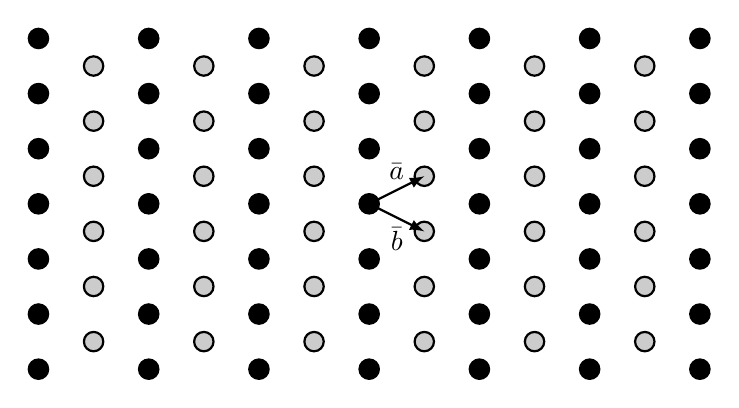
\begin{tikzpicture}[thick,scale=0.7]
\foreach \x in {2,4,...,14} {
    \foreach \y in {1,...,7} {
        \draw[draw=black,fill=black] (\x,\y) circle (5pt);
    }
}
\foreach \x in {3,5,...,13} {
    \foreach \y in {1.5,...,6.5} {
        \draw[draw=black,fill=black!20!white] (\x,\y) circle (5pt);
    }
}
\draw[-latex] (8,4)--(9,4.5) node[midway,above] {$\bar{a}$};
\draw[-latex] (8,4)--(9,3.5) node[midway,below] {$\bar{b}$};
\end{tikzpicture}

\caption{$P$ is a piece of the lattice generated by vectors $\bar{a}$ and $\bar{b}$.}
\end{figure}

The unit distance graph $G$ defined on these points is a matchstick graph and it has $n$ vertices and 
$e=\left(2-5/r-o(1)\right)n$ edges. 
\end{proof}

We continue with the upper bound in Theorem \ref{boundedmatchstick}.
Let $G$ be a matchstick graph on $n$ vertices in $D$.
A triangular face has area $\sqrt{3}/4$ and the area of $D$ is $r^2\pi$, therefore, 
there are at most $4r^2\pi/\sqrt{3}<8r^2$ triangular faces.
Remove an edge from the boundary of each triangle. The resulting matchstick graph $G'$ does not contain any triangle. 

Let $R$ be a rhombus face of $G'$.   
Suppose that its angles  are $\theta\le\pi/2$ and $\pi-\theta$. 
If $\theta\ge\pi/(50r^2)$, then it is called a \emph{fat rhombus}.




Each fat rhombus has area at least $\sin(\pi/(50r^2))\ge \pi/(100r^2)$. 
Therefore, there are at most $100r^4$ fat rhombi. Remove an edge from the boundary of each fat rhombus and let $G''$ be the resulting graph. 
The graph $G''$ does not contain a triangle or a fat rhombus and we have $e(G)\le e(G'')+100r^4+8r^2$. Let $e=e(G'')$.


\smallskip

Let $N$ be the \emph{neighborhood graph} of $G''$. The vertices of $N$ 
correspond to the edges of $G''$. 
Two vertices, $v_1\neq v_2$ are connected in $N$ if the corresponding edges are on the boundary of 
the same face. So each edge of $N$ corresponds to a face of $G''$.
For any edges $\alpha$ and $\beta$ of $G''$, we say that they are neighbors (resp.\ at distance $m$) if the corresponding
vertices, $v(\alpha)$ and $v(\beta)$ are neighbors (resp.\ at distance $m$) in $N$. Note that $N$ is the line graph of the dual graph of $G''$.

We say that an edge of $G''$ is \emph{irregular} if it is adjacent to a face which is not a rhombus, otherwise we call it \emph{regular}. 

\begin{lemma}\label{monopath}
Any regular edge has an irregular edge at distance at most $16r^2$.
\end{lemma} 

\smallskip


Before proving Lemma \ref{monopath}, we finish the proof of Theorem \ref{boundedmatchstick}. 
Let $e^*$ denote the number of irregular edges of $G''$. 
Let $f_i$ be the number of faces with $i$ boundary edges in $G''$.
By the definition of irregular edges, we have $2e-4f_4 \geq e^*$.

\smallskip
By (3), we have 
\begin{equation}\label{eq:e^*}
e=2n-4-\frac{1}{2}\sum\limits_{i\geq 5}(i-4)f_i
< 2n-\frac{1}{2}\sum\limits_{i\geq 5}\frac{i}{5}f_i
= 2n- \frac{1}{10} (2e-4f_4)
\le 2n-\frac{e^*}{10}.
\end{equation}



For each regular edge $\alpha$, assign one of the \emph{closest} irregular edges
$\epsilon(\alpha)$.
By Lemma \ref{monopath} 
we know that the distance between 
$\alpha$ and $\epsilon(\alpha)$ is at most $16r^2$, and in the shortest path 
between $v(\alpha)$ and $v(\epsilon(\alpha))$ in $N$  
all edges correspond to rhombi. 
\smallskip

Now we estimate the number of edges $\beta$ with the same assigned edge, that is, 
$\epsilon(\beta)=\epsilon(\alpha)$. 
For any such $\beta$ there is a path of length at most $16r^2$ from $\epsilon(\alpha)$ to $\beta$ 
all of whose edges correspond to rhombi. To build such a path, at each vertex we have three choices
to continue, corresponding to the other three sides of the rhombus. 
Thus, we have at most $\sum_{i=1}^{16r^2}3^i<2\cdot 3^{16r^2}$ different paths ending at $\epsilon(\alpha)$. Therefore, for the number of irregular edges $e^*$ we have
$2\cdot 3^{16r^2}e'\ge e-e^*$, so \[e^*\ge \frac{e}{4\cdot 3^{16r^2}}.\]
Consequently, by \eqref{eq:e^*}, we have
\begin{align*}
    e &\le 2n-4-\frac{e}{40\cdot 3^{16r^2}}\\
    e &\le \left(2-\frac{1}{20\cdot 3^{16r^2}} \right)n.
\end{align*}

Finally,
\[e(G)\le \left(2-\frac{1}{20\cdot 3^{16r^2}} \right)n+100r^4+8r^2.\]




\qed

\begin{proof}[Proof of the Lemma \ref{monopath}]
Suppose for a contradiction that there is an edge $\alpha$ 
with the property that its $16r^2$-neighborhood contains only regular edges. Without loss of generality we can assume that $\alpha$ is horizontal; otherwise, we rotate the drawing of $G''$.
\smallskip

A \emph{monotone path} is a path in $G''$ that intersects any vertical line at most once. 
Let $P$ be a monotone path in $G''$ and suppose that $R$ is a 
rhombus-face whose lower left and lower right edges are in $P$. Then $R$ is called a \emph{hat} on $P$. 
\smallskip

We apply the following procedure which builds a monotone path.

\bigskip


\textsc{Algorithm Extend-Path($\alpha$)}

\smallskip

\noindent \textsc{Step $0$.} Let $P_1$ be the path of length $1$ that consists of the edge $\alpha$.
Set $i=2$.


\smallskip

For $i=2, \ldots, $ we do the following.

\noindent \textsc{Step $(i, \, 1)$}. We have $i\ge 2$. 
Suppose that we already have a monotone path $P_{i-1}$.

If there is a \emph{hat} $H$ on it, then replace its two lower edges by its two upper edges in $P_{i-1}$. Let $P_{i-1}$ be the resulting monotone path.
Repeat \textsc{Step $(i, \, 1)$}.

If there is no hat on $P_{i-1}$, then go to \textsc{Step $(i, \, 2)$}.

\smallskip

\noindent \textsc{Step $(i, \, 2)$}. We have a monotone path $P_{i-1}$ of length $i-1$ with no hat on it.
Let $p_0, \, p_1, \, \ldots, \, p_i$ be the vertices of $P_{i-1}$ from left to right and let $F_j$ be the face on the upper side of 
$\epsilon_j=p_{j-1}p_j$. If $F_j$ is not a rhombus, then $\epsilon_j$ is an irregular edge. Let $\epsilon=\epsilon_j$ and {\textbf{Stop.}} \textbf{Return $(\epsilon, \, P_{i-1})$}.

\smallskip
We can assume now that all $F_j$ are rhombi and all of them are different. 
For every $j$, $\epsilon_j$ 
is \emph{rightsided} (resp.\ \emph{leftsided})
if $\epsilon_j$ is the lower \emph{right} (resp.\ lower \emph{left}) side of $F_j$. 
If $\epsilon_1$ is \emph{rightsided}, 
then $P_{i-1}$ can be extended by the lower left edge of $F_1$ to a monotone path $P_i$ 
of length $i$. Let  
$P_{i}$ be this path. Increase $i$ by one and go to \textsc{Step $(i, \, 1)$}.

Now we can assume that $\epsilon_1$ is \emph{leftsided}. 
But then $\epsilon_2$ is also \emph{leftsided}, otherwise 
$F_1$ and $F_2$ would both contain the points slightly above $p_1$, which is impossible since they
internally disjoint. By repeated application of the same argument, we get that all edges 
$\epsilon_1, \, \epsilon_2, \, \ldots, \, \epsilon_{i-1}$ are \emph{leftsided}.

So $\epsilon_{i-1}$ is 
\emph{leftsided},
therefore, $P_{i-1}$ can be extended by the lower right  
edge of $F_{i-1}$ to a monotone path $P_i$ 
of length $i$. Let  
$P_{i}$ be this path. 
Increase $i$  by one and go to \textsc{Step $(i, \, 1)$}.


\bigskip


\begin{definition}
For any monotone path $P$ of 
length $l$, let $c(P)$ denote the \emph{convexity number} of $P$.
It is defined as the number of pairs of edges 
$(\epsilon_1, \epsilon_2)$ of $P$ with the property that 
$\epsilon_1$ is to the left of $\epsilon_2$, and $\epsilon_1$ has smaller slope than $\epsilon_2$.
\end{definition} 

\smallskip

So, for any monotone path $P$ of length $l$, we have
$0\le c(P)\le \binom{l}{2}$. If 
$c(P)=0$, then $P$ is convex from below, if 
$c(P)=\binom{l}{2}$, then 
it is convex from above.

\textsc{Algorithm Extend-Path($\alpha$)}
will terminate after a finite number of steps, since $G''$ contains no monotone path longer than $n$.

Suppose hat the algorithm returns edge $\epsilon$ and path $P_l$ of length $l$.
We distinguish two cases. 

\smallskip

\noindent \textbf{Case 1:} $l\le 4r$.
The algorithm stopped in \textsc{Step $(l+1, \, 2)$}.  

For 
$1\le i\le l+1$, let $s(i)$ be the number of 
times 
\textsc{Step $(i,  \, 1)$} 
was executed. 
Observe that in each step, $c(P)$ decreases by one.
On the other hand, in \textsc{Step $(i,  \, 2)$}, when we construct 
$P_i$ from $P_{i-1}$, we have $c(P_i)\le c(P_{i-1})+i-1.$
Therefore, $$\sum_{i=1}^{l+1}s(i)\le \sum_{i=1}^{l+1}(i-1)<l(l+1)/2.$$ 
Consequently, the total number of steps executed by the algorithm is at most $l(l+1)/2+l\le 16r^2$. 
Thus, 
all edges of $P_{l}$, including $\epsilon$, are  
at distance at most $16r^2$ from $\alpha$, contradicting our assumption that $\epsilon$ is an irregular edge. 

\smallskip


\noindent \textbf{Case 2:} $l\ge 4r$. For $i=4r$, the algorithm  constructed $P_{4r}$, a monotone path of length $4r$.

Again, for $1\le i\le 4r$, let $s(i)$ be the number of times \textsc{Step $(i,  \, 1)$} was executed. By the same argument as in Case 1, we obtain that 
$$\sum_{i=1}^{4r}s(i)\le \sum_{i=1}^{4r}(i-1)<4r(4r-1)/2.$$
Consequently, the total number of steps executed by the algorithm is at most $4r(4r-1)/2+4r<16r^2$. Therefore, 
all edges of $P_{4r}$ are at distance at most $16r^2$ from $\alpha$. By the assumption that there is no irregular edge in the 
$16r^2$-neighborhood of $\alpha$, we conclude that from $\alpha$ to any edge of $P$, there is a sequence of adjacent rhombi, of length at most $16r^2$. 

We also assumed that there is no fat rhombus. Therefore, two edges of a rhombus determine an angle at most $\pi/50r^2$. It follows that the angle between $\alpha$ and any edge of $P_{4r}$ is less than $16r^2\pi/50r^2< \pi/3$. Consequently, the length of the projection of every edge of $P_{4r}$ to the $x$-axis is longer than $1/2$, so the projection of $P_{4r}$ to the $x$-axis is longer than $2r$. This contradicts the fact that $P_{4r}$ lies entirely in $D$, a disk of radius $r$. This concludes the proof of the Lemma. \end{proof}

\smallskip



\section{Concluding remarks}
\begin{enumerate}
\item We conjecture that the maximum number of edges in a triangle-free matchstick graph is at most $2n-\sqrt{2n}+O(1)$, maybe even exactly $\left\lfloor 2n-\sqrt{2n-\frac{7}{4}}-\frac{3}{2}\right\rfloor$ for every $n\geq 1$, which would show that the lower bound in Proposition~\ref{prop:triangle-free-lower-bound} is tight.

\item
Can our result for triangle-free matchstick graphs be generalized to graphs of higher girth?
Euler's formula implies that in a planar graph of 
$n$ vertices and 
girth $g$, the number of edges $e$ is bounded above by $e\le \frac{g}{g-2}(n-2)$.
It is natural to ask whether we have the stronger bound
$e\le \frac{g}{g-2}(n-2)-c(g)\sqrt{n}$ for matchstick graphs of girth $g\geq 5$, where $c(g) > 0$.
This is in fact easy to prove for odd $g$ using the isoperimetric inequality, since it is known that a simple polygon with an odd number of sides, all of unit length, has an area not smaller than that of a unit-length equilateral triangle \cite{BKM99}.
Do we get the same bound for even $g\geq 6$?

\item 
Improve the bounds in Theorem~\ref{boundedmatchstick}.
Is it true that $e_r(n)=(2-c(r))n$ for some $c(r)=\Theta(1/r)$?
\end{enumerate}


\vspace{5mm}

\noindent
{\bf \large Acknowledgments.}
Panna Geh\'er, J\'anos Pach and G\'eza T\'oth were supported by ERC Advanced Grant `GeoScape' No.\ 882971 and by the National Research, Development and Innovation Office, NKFIH, K-131529. J\'anos Pach was also supported by NSF Grant DMS-1928930, while he was in residence at SLMath Berkeley, during the Spring 2025 semester.
Konrad Swanepoel was partially supported by ERC Advanced Grant `GeoScape' No.\ 882971 and by the Erd\H os Center.


\begin{thebibliography}{20}

\bibitem{BKM99}
B\"or\"oczky, K., Kert\'esz, G., Makai, E.\ Jr.\ (1999).
\emph{The minimum area of a simple polygon with given side lengths.}
Periodica Mathematica Hungarica, 39(1--3), 33--49.


\bibitem{E17}
Eppstein, D.\ (2017).
\emph{Triangle-free penny graphs: degeneracy, choosability, and edge count.}
In International Symposium on Graph Drawing and Network Visualization (pp.\ 506--513). Cham: Springer International Publishing.

\bibitem{E46}
Erd\H{o}s, P.\ (1946).
\emph{On sets of distances of $n$ points.}
The American Mathematical Monthly, 53(5), 248--250.


\bibitem{GT24}
Geh\'er, P., T\'oth, G.\ (2024).
\emph{1-planar unit distance graphs.}
In 32nd International Symposium on Graph Drawing and Network Visualization. Leibniz International Proceedings in Informatics (LIPIcs), Vol.\ 320, pp.\ 6:1--6:9, Schloss Dagstuhl - Leibniz-Zentrum für Informatik.

\bibitem{Harborth74}
Harborth, H.\ (1974).
\emph{Solution to problem 664A.}
Elemente der Mathematik, 29, 14--15.

\bibitem{Harborth1}
Harborth, H.\ (1981).
\emph{Point sets with equal numbers of unit-distant neighbors.}
(Abstract),
Discrete Geometry, 12--18 July 1981, Oberwolfach,
Tagungsbericht 31/1981, Mathematisches Forschungsinstitut Oberwolfach. pp.~11--12.

\bibitem{Harborth2}
Harborth, H.\ (1994).
\emph{Match sticks in the plane.}
In The Lighter Side of Mathematics.
Proceedings of the Eug\`ene Strens Memorial Conference on Recreational Mathematics and its History held at the University of Calgary, Calgary, Alberta, August 1986., edited by R.\ K.\ Guy and R.\ E.\ Woodrow, 281--288. Mathematical Association of America, Washington, D.C.

\bibitem{KS92}
Kannan, S., Soroker, D.\ (1992).
\emph{Tiling polygons with parallelograms.}
Discrete and Computational Geometry, 7(2), 175--188.

\bibitem{K93}
Kenyon, R.\ (1993).
\emph{Tiling a polygon with parallelograms.}
Algorithmica, 9, 382--397.


\bibitem{LS22}
Lavoll\'ee, J., Swanepoel, K.\ J.\ (2024).
\emph{A tight bound for the number of edges of matchstick graphs.}
Discrete and Computational Geometry, 72(4), 1530--1544.


\bibitem{S09}
Swanepoel, K.\ J.\ (2009).
\emph{Triangle-free minimum distance graphs in the plane.}
Geombinatorics, 19(1), 28--30.



\end{thebibliography}
\end{document}





